\documentclass[twoside]{book}

% Packages required by doxygen
\usepackage{fixltx2e}
\usepackage{calc}
\usepackage{doxygen}
\usepackage[export]{adjustbox} % also loads graphicx
\usepackage{graphicx}
\usepackage[utf8]{inputenc}
\usepackage{makeidx}
\usepackage{multicol}
\usepackage{multirow}
\PassOptionsToPackage{warn}{textcomp}
\usepackage{textcomp}
\usepackage[nointegrals]{wasysym}
\usepackage[table]{xcolor}

% Font selection
\usepackage[T1]{fontenc}
\usepackage[scaled=.90]{helvet}
\usepackage{courier}
\usepackage{amssymb}
\usepackage{sectsty}
\renewcommand{\familydefault}{\sfdefault}
\allsectionsfont{%
  \fontseries{bc}\selectfont%
  \color{darkgray}%
}
\renewcommand{\DoxyLabelFont}{%
  \fontseries{bc}\selectfont%
  \color{darkgray}%
}
\newcommand{\+}{\discretionary{\mbox{\scriptsize$\hookleftarrow$}}{}{}}

% Page & text layout
\usepackage{geometry}
\geometry{%
  a4paper,%
  top=2.5cm,%
  bottom=2.5cm,%
  left=2.5cm,%
  right=2.5cm%
}
\tolerance=750
\hfuzz=15pt
\hbadness=750
\setlength{\emergencystretch}{15pt}
\setlength{\parindent}{0cm}
\setlength{\parskip}{3ex plus 2ex minus 2ex}
\makeatletter
\renewcommand{\paragraph}{%
  \@startsection{paragraph}{4}{0ex}{-1.0ex}{1.0ex}{%
    \normalfont\normalsize\bfseries\SS@parafont%
  }%
}
\renewcommand{\subparagraph}{%
  \@startsection{subparagraph}{5}{0ex}{-1.0ex}{1.0ex}{%
    \normalfont\normalsize\bfseries\SS@subparafont%
  }%
}
\makeatother

% Headers & footers
\usepackage{fancyhdr}
\pagestyle{fancyplain}
\fancyhead[LE]{\fancyplain{}{\bfseries\thepage}}
\fancyhead[CE]{\fancyplain{}{}}
\fancyhead[RE]{\fancyplain{}{\bfseries\leftmark}}
\fancyhead[LO]{\fancyplain{}{\bfseries\rightmark}}
\fancyhead[CO]{\fancyplain{}{}}
\fancyhead[RO]{\fancyplain{}{\bfseries\thepage}}
\fancyfoot[LE]{\fancyplain{}{}}
\fancyfoot[CE]{\fancyplain{}{}}
\fancyfoot[RE]{\fancyplain{}{\bfseries\scriptsize Generated by Doxygen }}
\fancyfoot[LO]{\fancyplain{}{\bfseries\scriptsize Generated by Doxygen }}
\fancyfoot[CO]{\fancyplain{}{}}
\fancyfoot[RO]{\fancyplain{}{}}
\renewcommand{\footrulewidth}{0.4pt}
\renewcommand{\chaptermark}[1]{%
  \markboth{#1}{}%
}
\renewcommand{\sectionmark}[1]{%
  \markright{\thesection\ #1}%
}

% Indices & bibliography
\usepackage{natbib}
\usepackage[titles]{tocloft}
\setcounter{tocdepth}{3}
\setcounter{secnumdepth}{5}
\makeindex

% Hyperlinks (required, but should be loaded last)
\usepackage{ifpdf}
\ifpdf
  \usepackage[pdftex,pagebackref=true]{hyperref}
\else
  \usepackage[ps2pdf,pagebackref=true]{hyperref}
\fi
\hypersetup{%
  colorlinks=true,%
  linkcolor=blue,%
  citecolor=blue,%
  unicode%
}

% Custom commands
\newcommand{\clearemptydoublepage}{%
  \newpage{\pagestyle{empty}\cleardoublepage}%
}

\usepackage{caption}
\captionsetup{labelsep=space,justification=centering,font={bf},singlelinecheck=off,skip=4pt,position=top}

%===== C O N T E N T S =====

\begin{document}

% Titlepage & ToC
\hypersetup{pageanchor=false,
             bookmarksnumbered=true,
             pdfencoding=unicode
            }
\pagenumbering{alph}
\begin{titlepage}
\vspace*{7cm}
\begin{center}%
{\Large 09-\/bayan }\\
\vspace*{1cm}
{\large Generated by Doxygen 1.8.13}\\
\end{center}
\end{titlepage}
\clearemptydoublepage
\pagenumbering{roman}
\tableofcontents
\clearemptydoublepage
\pagenumbering{arabic}
\hypersetup{pageanchor=true}

%--- Begin generated contents ---
\chapter{Namespace Index}
\section{Namespace List}
Here is a list of all namespaces with brief descriptions\+:\begin{DoxyCompactList}
\item\contentsline{section}{\hyperlink{namespacematrix}{matrix} }{\pageref{namespacematrix}}{}
\item\contentsline{section}{\hyperlink{namespacematrix_1_1detail}{matrix\+::detail} }{\pageref{namespacematrix_1_1detail}}{}
\end{DoxyCompactList}

\chapter{Hierarchical Index}
\section{Class Hierarchy}
This inheritance list is sorted roughly, but not completely, alphabetically\+:\begin{DoxyCompactList}
\item \contentsline{section}{bayan\+:\+:hash\+:\+:hash}{\pageref{classbayan_1_1hash_1_1hash}}{}
\begin{DoxyCompactList}
\item \contentsline{section}{bayan\+:\+:hash\+:\+:md5}{\pageref{classbayan_1_1hash_1_1md5}}{}
\end{DoxyCompactList}
\item \contentsline{section}{bayan\+:\+:options}{\pageref{structbayan_1_1options}}{}
\end{DoxyCompactList}

\chapter{Class Index}
\section{Class List}
Here are the classes, structs, unions and interfaces with brief descriptions\+:\begin{DoxyCompactList}
\item\contentsline{section}{\hyperlink{classedu__allocator}{edu\+\_\+allocator$<$ T, batch\+\_\+count $>$} }{\pageref{classedu__allocator}}{}
\item\contentsline{section}{\hyperlink{classedu__container}{edu\+\_\+container$<$ T, size, Alloc $>$} }{\pageref{classedu__container}}{}
\item\contentsline{section}{\hyperlink{structedu__allocator_1_1rebind}{edu\+\_\+allocator$<$ T, batch\+\_\+count $>$\+::rebind$<$ U $>$} }{\pageref{structedu__allocator_1_1rebind}}{}
\end{DoxyCompactList}

\chapter{File Index}
\section{File List}
Here is a list of all files with brief descriptions\+:\begin{DoxyCompactList}
\item\contentsline{section}{src/\hyperlink{block__printer_8cpp}{block\+\_\+printer.\+cpp} }{\pageref{block__printer_8cpp}}{}
\item\contentsline{section}{src/\hyperlink{block__printer_8hpp}{block\+\_\+printer.\+hpp} }{\pageref{block__printer_8hpp}}{}
\item\contentsline{section}{src/\hyperlink{block__reader_8cpp}{block\+\_\+reader.\+cpp} }{\pageref{block__reader_8cpp}}{}
\item\contentsline{section}{src/\hyperlink{block__reader_8hpp}{block\+\_\+reader.\+hpp} }{\pageref{block__reader_8hpp}}{}
\item\contentsline{section}{src/\hyperlink{line__reader_8cpp}{line\+\_\+reader.\+cpp} }{\pageref{line__reader_8cpp}}{}
\item\contentsline{section}{src/\hyperlink{line__reader_8hpp}{line\+\_\+reader.\+hpp} }{\pageref{line__reader_8hpp}}{}
\item\contentsline{section}{src/\hyperlink{main_8cpp}{main.\+cpp} }{\pageref{main_8cpp}}{}
\item\contentsline{section}{src/\hyperlink{observable_8hpp}{observable.\+hpp} }{\pageref{observable_8hpp}}{}
\end{DoxyCompactList}

\chapter{Namespace Documentation}
\hypertarget{namespacebayan}{}\section{bayan Namespace Reference}
\label{namespacebayan}\index{bayan@{bayan}}
\subsection*{Namespaces}
\begin{DoxyCompactItemize}
\item 
 \hyperlink{namespacebayan_1_1hash}{hash}
\end{DoxyCompactItemize}
\subsection*{Classes}
\begin{DoxyCompactItemize}
\item 
struct \hyperlink{structbayan_1_1options}{options}
\end{DoxyCompactItemize}
\subsection*{Functions}
\begin{DoxyCompactItemize}
\item 
\hyperlink{structbayan_1_1options}{options} \hyperlink{namespacebayan_aa357fd1ddce71ed465f7fa6bd8f8f2e3}{parse\+\_\+options} (int argc, const char $\ast$$\ast$argv)
\end{DoxyCompactItemize}


\subsection{Function Documentation}
\mbox{\Hypertarget{namespacebayan_aa357fd1ddce71ed465f7fa6bd8f8f2e3}\label{namespacebayan_aa357fd1ddce71ed465f7fa6bd8f8f2e3}} 
\index{bayan@{bayan}!parse\+\_\+options@{parse\+\_\+options}}
\index{parse\+\_\+options@{parse\+\_\+options}!bayan@{bayan}}
\subsubsection{\texorpdfstring{parse\+\_\+options()}{parse\_options()}}
{\footnotesize\ttfamily \hyperlink{structbayan_1_1options}{bayan\+::options} bayan\+::parse\+\_\+options (\begin{DoxyParamCaption}\item[{int}]{argc,  }\item[{const char $\ast$$\ast$}]{argv }\end{DoxyParamCaption})}


\hypertarget{namespacebayan_1_1hash}{}\section{bayan\+:\+:hash Namespace Reference}
\label{namespacebayan_1_1hash}\index{bayan\+::hash@{bayan\+::hash}}
\subsection*{Classes}
\begin{DoxyCompactItemize}
\item 
class \hyperlink{classbayan_1_1hash_1_1hash}{hash}
\item 
class \hyperlink{classbayan_1_1hash_1_1md5}{md5}
\end{DoxyCompactItemize}
\subsection*{Functions}
\begin{DoxyCompactItemize}
\item 
std\+::unique\+\_\+ptr$<$ \hyperlink{classbayan_1_1hash_1_1hash}{hash} $>$ \hyperlink{namespacebayan_1_1hash_a9cd51387d3f16f6a1e7c76c47ee00a3b}{create\+\_\+hash} (std\+::string\+\_\+view algorithm)
\end{DoxyCompactItemize}


\subsection{Function Documentation}
\mbox{\Hypertarget{namespacebayan_1_1hash_a9cd51387d3f16f6a1e7c76c47ee00a3b}\label{namespacebayan_1_1hash_a9cd51387d3f16f6a1e7c76c47ee00a3b}} 
\index{bayan\+::hash@{bayan\+::hash}!create\+\_\+hash@{create\+\_\+hash}}
\index{create\+\_\+hash@{create\+\_\+hash}!bayan\+::hash@{bayan\+::hash}}
\subsubsection{\texorpdfstring{create\+\_\+hash()}{create\_hash()}}
{\footnotesize\ttfamily std\+::unique\+\_\+ptr$<$ \hyperlink{classbayan_1_1hash_1_1hash}{hash} $>$ bayan\+::hash\+::create\+\_\+hash (\begin{DoxyParamCaption}\item[{std\+::string\+\_\+view}]{algorithm }\end{DoxyParamCaption})}


\chapter{Class Documentation}
\hypertarget{classbayan_1_1hash_1_1hash}{}\section{bayan\+:\+:hash\+:\+:hash Class Reference}
\label{classbayan_1_1hash_1_1hash}\index{bayan\+::hash\+::hash@{bayan\+::hash\+::hash}}


{\ttfamily \#include $<$hash.\+hpp$>$}

Inheritance diagram for bayan\+:\+:hash\+:\+:hash\+:\begin{figure}[H]
\begin{center}
\leavevmode
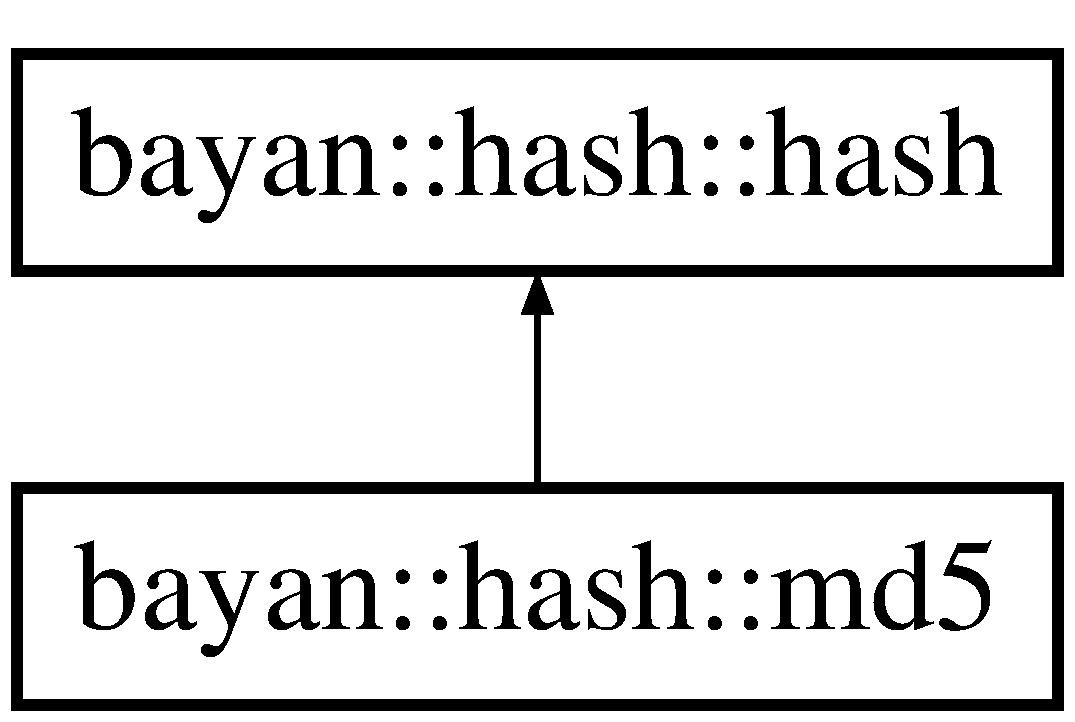
\includegraphics[height=2.000000cm]{classbayan_1_1hash_1_1hash}
\end{center}
\end{figure}
\subsection*{Public Member Functions}
\begin{DoxyCompactItemize}
\item 
virtual \hyperlink{classbayan_1_1hash_1_1hash_a115b320d7c70ffdd24e8df2fa2a1e892}{$\sim$hash} ()=default
\item 
virtual void \hyperlink{classbayan_1_1hash_1_1hash_abc43a44f53acc0278f46a96438dc4cf3}{update} (const char $\ast$data, size\+\_\+t size)=0
\item 
virtual std\+::vector$<$ uint8\+\_\+t $>$ \hyperlink{classbayan_1_1hash_1_1hash_a0532214ff924522ba61fbe9a6ade4705}{finish} ()=0
\end{DoxyCompactItemize}


\subsection{Constructor \& Destructor Documentation}
\mbox{\Hypertarget{classbayan_1_1hash_1_1hash_a115b320d7c70ffdd24e8df2fa2a1e892}\label{classbayan_1_1hash_1_1hash_a115b320d7c70ffdd24e8df2fa2a1e892}} 
\index{bayan\+::hash\+::hash@{bayan\+::hash\+::hash}!````~hash@{$\sim$hash}}
\index{````~hash@{$\sim$hash}!bayan\+::hash\+::hash@{bayan\+::hash\+::hash}}
\subsubsection{\texorpdfstring{$\sim$hash()}{~hash()}}
{\footnotesize\ttfamily virtual bayan\+::hash\+::hash\+::$\sim$hash (\begin{DoxyParamCaption}{ }\end{DoxyParamCaption})\hspace{0.3cm}{\ttfamily [virtual]}, {\ttfamily [default]}}



\subsection{Member Function Documentation}
\mbox{\Hypertarget{classbayan_1_1hash_1_1hash_a0532214ff924522ba61fbe9a6ade4705}\label{classbayan_1_1hash_1_1hash_a0532214ff924522ba61fbe9a6ade4705}} 
\index{bayan\+::hash\+::hash@{bayan\+::hash\+::hash}!finish@{finish}}
\index{finish@{finish}!bayan\+::hash\+::hash@{bayan\+::hash\+::hash}}
\subsubsection{\texorpdfstring{finish()}{finish()}}
{\footnotesize\ttfamily virtual std\+::vector$<$uint8\+\_\+t$>$ bayan\+::hash\+::hash\+::finish (\begin{DoxyParamCaption}{ }\end{DoxyParamCaption})\hspace{0.3cm}{\ttfamily [pure virtual]}}



Implemented in \hyperlink{classbayan_1_1hash_1_1md5_ade79012c138da38c8b08555dd48f637d}{bayan\+::hash\+::md5}.

\mbox{\Hypertarget{classbayan_1_1hash_1_1hash_abc43a44f53acc0278f46a96438dc4cf3}\label{classbayan_1_1hash_1_1hash_abc43a44f53acc0278f46a96438dc4cf3}} 
\index{bayan\+::hash\+::hash@{bayan\+::hash\+::hash}!update@{update}}
\index{update@{update}!bayan\+::hash\+::hash@{bayan\+::hash\+::hash}}
\subsubsection{\texorpdfstring{update()}{update()}}
{\footnotesize\ttfamily virtual void bayan\+::hash\+::hash\+::update (\begin{DoxyParamCaption}\item[{const char $\ast$}]{data,  }\item[{size\+\_\+t}]{size }\end{DoxyParamCaption})\hspace{0.3cm}{\ttfamily [pure virtual]}}



Implemented in \hyperlink{classbayan_1_1hash_1_1md5_abfa472bb4db577181800004c0996236f}{bayan\+::hash\+::md5}.



The documentation for this class was generated from the following file\+:\begin{DoxyCompactItemize}
\item 
src/hash/\hyperlink{hash_8hpp}{hash.\+hpp}\end{DoxyCompactItemize}

\hypertarget{classbayan_1_1hash_1_1md5}{}\section{bayan\+:\+:hash\+:\+:md5 Class Reference}
\label{classbayan_1_1hash_1_1md5}\index{bayan\+::hash\+::md5@{bayan\+::hash\+::md5}}


{\ttfamily \#include $<$md5.\+hpp$>$}

Inheritance diagram for bayan\+:\+:hash\+:\+:md5\+:\begin{figure}[H]
\begin{center}
\leavevmode
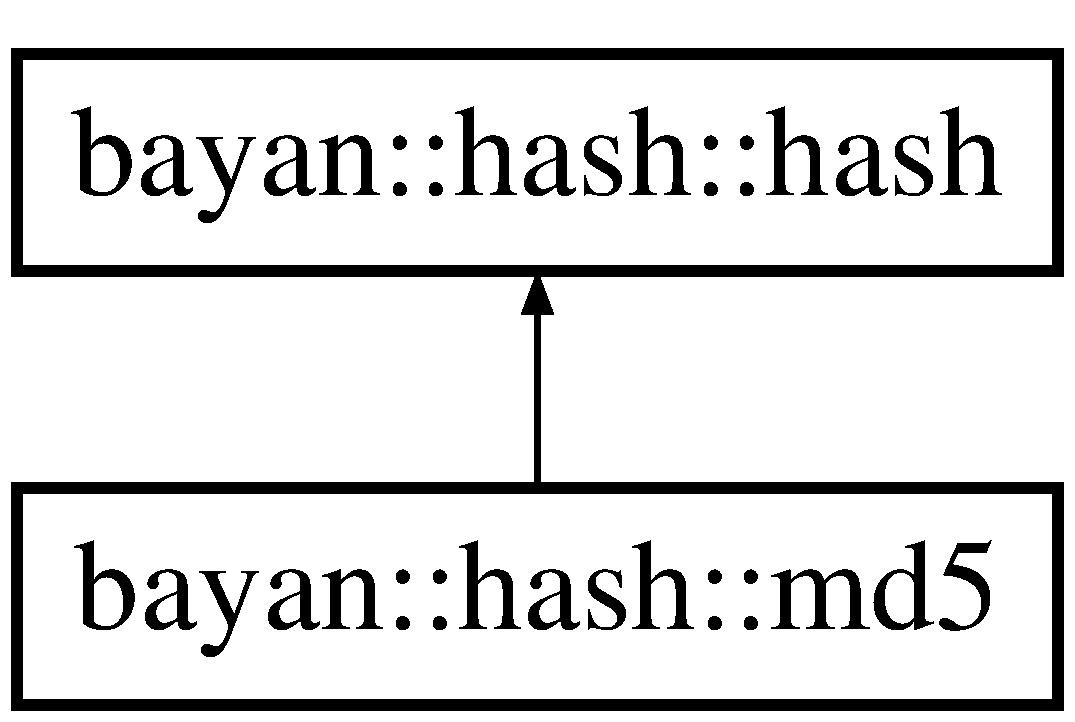
\includegraphics[height=2.000000cm]{classbayan_1_1hash_1_1md5}
\end{center}
\end{figure}
\subsection*{Public Member Functions}
\begin{DoxyCompactItemize}
\item 
\hyperlink{classbayan_1_1hash_1_1md5_a387a2c50afbcf62d3601a5436d3b7331}{md5} ()
\item 
\hyperlink{classbayan_1_1hash_1_1md5_a76f7a0803576bd2746bca20a985407c4}{$\sim$md5} () override=default
\item 
void \hyperlink{classbayan_1_1hash_1_1md5_abfa472bb4db577181800004c0996236f}{update} (const char $\ast$data, size\+\_\+t size) override
\item 
std\+::vector$<$ uint8\+\_\+t $>$ \hyperlink{classbayan_1_1hash_1_1md5_ade79012c138da38c8b08555dd48f637d}{finish} () override
\end{DoxyCompactItemize}


\subsection{Constructor \& Destructor Documentation}
\mbox{\Hypertarget{classbayan_1_1hash_1_1md5_a387a2c50afbcf62d3601a5436d3b7331}\label{classbayan_1_1hash_1_1md5_a387a2c50afbcf62d3601a5436d3b7331}} 
\index{bayan\+::hash\+::md5@{bayan\+::hash\+::md5}!md5@{md5}}
\index{md5@{md5}!bayan\+::hash\+::md5@{bayan\+::hash\+::md5}}
\subsubsection{\texorpdfstring{md5()}{md5()}}
{\footnotesize\ttfamily bayan\+::hash\+::md5\+::md5 (\begin{DoxyParamCaption}{ }\end{DoxyParamCaption})}

\mbox{\Hypertarget{classbayan_1_1hash_1_1md5_a76f7a0803576bd2746bca20a985407c4}\label{classbayan_1_1hash_1_1md5_a76f7a0803576bd2746bca20a985407c4}} 
\index{bayan\+::hash\+::md5@{bayan\+::hash\+::md5}!````~md5@{$\sim$md5}}
\index{````~md5@{$\sim$md5}!bayan\+::hash\+::md5@{bayan\+::hash\+::md5}}
\subsubsection{\texorpdfstring{$\sim$md5()}{~md5()}}
{\footnotesize\ttfamily bayan\+::hash\+::md5\+::$\sim$md5 (\begin{DoxyParamCaption}{ }\end{DoxyParamCaption})\hspace{0.3cm}{\ttfamily [override]}, {\ttfamily [default]}}



\subsection{Member Function Documentation}
\mbox{\Hypertarget{classbayan_1_1hash_1_1md5_ade79012c138da38c8b08555dd48f637d}\label{classbayan_1_1hash_1_1md5_ade79012c138da38c8b08555dd48f637d}} 
\index{bayan\+::hash\+::md5@{bayan\+::hash\+::md5}!finish@{finish}}
\index{finish@{finish}!bayan\+::hash\+::md5@{bayan\+::hash\+::md5}}
\subsubsection{\texorpdfstring{finish()}{finish()}}
{\footnotesize\ttfamily std\+::vector$<$ uint8\+\_\+t $>$ bayan\+::hash\+::md5\+::finish (\begin{DoxyParamCaption}{ }\end{DoxyParamCaption})\hspace{0.3cm}{\ttfamily [override]}, {\ttfamily [virtual]}}



Implements \hyperlink{classbayan_1_1hash_1_1hash_a0532214ff924522ba61fbe9a6ade4705}{bayan\+::hash\+::hash}.

\mbox{\Hypertarget{classbayan_1_1hash_1_1md5_abfa472bb4db577181800004c0996236f}\label{classbayan_1_1hash_1_1md5_abfa472bb4db577181800004c0996236f}} 
\index{bayan\+::hash\+::md5@{bayan\+::hash\+::md5}!update@{update}}
\index{update@{update}!bayan\+::hash\+::md5@{bayan\+::hash\+::md5}}
\subsubsection{\texorpdfstring{update()}{update()}}
{\footnotesize\ttfamily void bayan\+::hash\+::md5\+::update (\begin{DoxyParamCaption}\item[{const char $\ast$}]{data,  }\item[{size\+\_\+t}]{size }\end{DoxyParamCaption})\hspace{0.3cm}{\ttfamily [override]}, {\ttfamily [virtual]}}



Implements \hyperlink{classbayan_1_1hash_1_1hash_abc43a44f53acc0278f46a96438dc4cf3}{bayan\+::hash\+::hash}.



The documentation for this class was generated from the following files\+:\begin{DoxyCompactItemize}
\item 
src/hash/\hyperlink{md5_8hpp}{md5.\+hpp}\item 
src/hash/\hyperlink{md5_8cpp}{md5.\+cpp}\end{DoxyCompactItemize}

\hypertarget{structbayan_1_1options}{}\section{bayan\+:\+:options Struct Reference}
\label{structbayan_1_1options}\index{bayan\+::options@{bayan\+::options}}


{\ttfamily \#include $<$options.\+hpp$>$}

\subsection*{Public Attributes}
\begin{DoxyCompactItemize}
\item 
std\+::vector$<$ boost\+::filesystem\+::path $>$ \hyperlink{structbayan_1_1options_a70d39c9cc1e3f0abbed5120bf4f905a8}{include} \{\}
\item 
std\+::vector$<$ boost\+::filesystem\+::path $>$ \hyperlink{structbayan_1_1options_a502a24e54aebe8dc1ff92dda9b051874}{exclude} \{\}
\item 
size\+\_\+t \hyperlink{structbayan_1_1options_a388ae65a4e37c117102246d331d35841}{depth} \{\}
\item 
size\+\_\+t \hyperlink{structbayan_1_1options_a04bf4ca814015adfba86f01e6201ca3c}{minimum\+\_\+size} \{\}
\item 
std\+::vector$<$ std\+::string $>$ \hyperlink{structbayan_1_1options_a9eaad24fb60c372c5f21b06e2d6bd051}{name\+\_\+masks} \{\}
\item 
size\+\_\+t \hyperlink{structbayan_1_1options_a933b3640331398d9c27b4e08790f8046}{block\+\_\+size} \{\}
\item 
std\+::string \hyperlink{structbayan_1_1options_a1eb16ba1d461fa60a519b902b00e35e0}{algorithm} \{\}
\end{DoxyCompactItemize}


\subsection{Member Data Documentation}
\mbox{\Hypertarget{structbayan_1_1options_a1eb16ba1d461fa60a519b902b00e35e0}\label{structbayan_1_1options_a1eb16ba1d461fa60a519b902b00e35e0}} 
\index{bayan\+::options@{bayan\+::options}!algorithm@{algorithm}}
\index{algorithm@{algorithm}!bayan\+::options@{bayan\+::options}}
\subsubsection{\texorpdfstring{algorithm}{algorithm}}
{\footnotesize\ttfamily std\+::string bayan\+::options\+::algorithm \{\}}

\mbox{\Hypertarget{structbayan_1_1options_a933b3640331398d9c27b4e08790f8046}\label{structbayan_1_1options_a933b3640331398d9c27b4e08790f8046}} 
\index{bayan\+::options@{bayan\+::options}!block\+\_\+size@{block\+\_\+size}}
\index{block\+\_\+size@{block\+\_\+size}!bayan\+::options@{bayan\+::options}}
\subsubsection{\texorpdfstring{block\+\_\+size}{block\_size}}
{\footnotesize\ttfamily size\+\_\+t bayan\+::options\+::block\+\_\+size \{\}}

\mbox{\Hypertarget{structbayan_1_1options_a388ae65a4e37c117102246d331d35841}\label{structbayan_1_1options_a388ae65a4e37c117102246d331d35841}} 
\index{bayan\+::options@{bayan\+::options}!depth@{depth}}
\index{depth@{depth}!bayan\+::options@{bayan\+::options}}
\subsubsection{\texorpdfstring{depth}{depth}}
{\footnotesize\ttfamily size\+\_\+t bayan\+::options\+::depth \{\}}

\mbox{\Hypertarget{structbayan_1_1options_a502a24e54aebe8dc1ff92dda9b051874}\label{structbayan_1_1options_a502a24e54aebe8dc1ff92dda9b051874}} 
\index{bayan\+::options@{bayan\+::options}!exclude@{exclude}}
\index{exclude@{exclude}!bayan\+::options@{bayan\+::options}}
\subsubsection{\texorpdfstring{exclude}{exclude}}
{\footnotesize\ttfamily std\+::vector$<$boost\+::filesystem\+::path$>$ bayan\+::options\+::exclude \{\}}

\mbox{\Hypertarget{structbayan_1_1options_a70d39c9cc1e3f0abbed5120bf4f905a8}\label{structbayan_1_1options_a70d39c9cc1e3f0abbed5120bf4f905a8}} 
\index{bayan\+::options@{bayan\+::options}!include@{include}}
\index{include@{include}!bayan\+::options@{bayan\+::options}}
\subsubsection{\texorpdfstring{include}{include}}
{\footnotesize\ttfamily std\+::vector$<$boost\+::filesystem\+::path$>$ bayan\+::options\+::include \{\}}

\mbox{\Hypertarget{structbayan_1_1options_a04bf4ca814015adfba86f01e6201ca3c}\label{structbayan_1_1options_a04bf4ca814015adfba86f01e6201ca3c}} 
\index{bayan\+::options@{bayan\+::options}!minimum\+\_\+size@{minimum\+\_\+size}}
\index{minimum\+\_\+size@{minimum\+\_\+size}!bayan\+::options@{bayan\+::options}}
\subsubsection{\texorpdfstring{minimum\+\_\+size}{minimum\_size}}
{\footnotesize\ttfamily size\+\_\+t bayan\+::options\+::minimum\+\_\+size \{\}}

\mbox{\Hypertarget{structbayan_1_1options_a9eaad24fb60c372c5f21b06e2d6bd051}\label{structbayan_1_1options_a9eaad24fb60c372c5f21b06e2d6bd051}} 
\index{bayan\+::options@{bayan\+::options}!name\+\_\+masks@{name\+\_\+masks}}
\index{name\+\_\+masks@{name\+\_\+masks}!bayan\+::options@{bayan\+::options}}
\subsubsection{\texorpdfstring{name\+\_\+masks}{name\_masks}}
{\footnotesize\ttfamily std\+::vector$<$std\+::string$>$ bayan\+::options\+::name\+\_\+masks \{\}}



The documentation for this struct was generated from the following file\+:\begin{DoxyCompactItemize}
\item 
src/\hyperlink{options_8hpp}{options.\+hpp}\end{DoxyCompactItemize}

\chapter{File Documentation}
\hypertarget{CMakeLists_8txt}{}\section{src/\+C\+Make\+Lists.txt File Reference}
\label{CMakeLists_8txt}\index{src/\+C\+Make\+Lists.\+txt@{src/\+C\+Make\+Lists.\+txt}}

\hypertarget{hash_2CMakeLists_8txt}{}\section{src/hash/\+C\+Make\+Lists.txt File Reference}
\label{hash_2CMakeLists_8txt}\index{src/hash/\+C\+Make\+Lists.\+txt@{src/hash/\+C\+Make\+Lists.\+txt}}

\hypertarget{hash_8cpp}{}\section{src/hash/hash.cpp File Reference}
\label{hash_8cpp}\index{src/hash/hash.\+cpp@{src/hash/hash.\+cpp}}
{\ttfamily \#include \char`\"{}hash.\+hpp\char`\"{}}\newline
{\ttfamily \#include \char`\"{}md5.\+hpp\char`\"{}}\newline

\hypertarget{hash_8hpp}{}\section{src/hash/hash.hpp File Reference}
\label{hash_8hpp}\index{src/hash/hash.\+hpp@{src/hash/hash.\+hpp}}
{\ttfamily \#include $<$cstdlib$>$}\newline
{\ttfamily \#include $<$vector$>$}\newline
{\ttfamily \#include $<$memory$>$}\newline
{\ttfamily \#include $<$string$>$}\newline
\subsection*{Classes}
\begin{DoxyCompactItemize}
\item 
class \hyperlink{classbayan_1_1hash_1_1hash}{bayan\+::hash\+::hash}
\end{DoxyCompactItemize}
\subsection*{Namespaces}
\begin{DoxyCompactItemize}
\item 
 \hyperlink{namespacebayan_1_1hash}{bayan\+::hash}
\end{DoxyCompactItemize}
\subsection*{Functions}
\begin{DoxyCompactItemize}
\item 
std\+::unique\+\_\+ptr$<$ \hyperlink{classbayan_1_1hash_1_1hash}{hash} $>$ \hyperlink{namespacebayan_1_1hash_a9cd51387d3f16f6a1e7c76c47ee00a3b}{bayan\+::hash\+::create\+\_\+hash} (std\+::string\+\_\+view algorithm)
\end{DoxyCompactItemize}

\hypertarget{md5_8cpp}{}\section{src/hash/md5.cpp File Reference}
\label{md5_8cpp}\index{src/hash/md5.\+cpp@{src/hash/md5.\+cpp}}
{\ttfamily \#include \char`\"{}md5.\+hpp\char`\"{}}\newline
{\ttfamily \#include $<$stdexcept$>$}\newline

\hypertarget{md5_8hpp}{}\section{src/hash/md5.hpp File Reference}
\label{md5_8hpp}\index{src/hash/md5.\+hpp@{src/hash/md5.\+hpp}}
{\ttfamily \#include \char`\"{}hash.\+hpp\char`\"{}}\newline
{\ttfamily \#include $<$openssl/md5.\+h$>$}\newline
\subsection*{Classes}
\begin{DoxyCompactItemize}
\item 
class \hyperlink{classbayan_1_1hash_1_1md5}{bayan\+::hash\+::md5}
\end{DoxyCompactItemize}
\subsection*{Namespaces}
\begin{DoxyCompactItemize}
\item 
 \hyperlink{namespacebayan_1_1hash}{bayan\+::hash}
\end{DoxyCompactItemize}

\hypertarget{main_8cpp}{}\section{src/main.cpp File Reference}
\label{main_8cpp}\index{src/main.\+cpp@{src/main.\+cpp}}
\subsection*{Functions}
\begin{DoxyCompactItemize}
\item 
int \hyperlink{main_8cpp_ae66f6b31b5ad750f1fe042a706a4e3d4}{main} ()
\end{DoxyCompactItemize}


\subsection{Function Documentation}
\mbox{\Hypertarget{main_8cpp_ae66f6b31b5ad750f1fe042a706a4e3d4}\label{main_8cpp_ae66f6b31b5ad750f1fe042a706a4e3d4}} 
\index{main.\+cpp@{main.\+cpp}!main@{main}}
\index{main@{main}!main.\+cpp@{main.\+cpp}}
\subsubsection{\texorpdfstring{main()}{main()}}
{\footnotesize\ttfamily int main (\begin{DoxyParamCaption}{ }\end{DoxyParamCaption})}


\hypertarget{options_8cpp}{}\section{src/options.cpp File Reference}
\label{options_8cpp}\index{src/options.\+cpp@{src/options.\+cpp}}
{\ttfamily \#include \char`\"{}options.\+hpp\char`\"{}}\newline
{\ttfamily \#include $<$boost/program\+\_\+options/options\+\_\+description.\+hpp$>$}\newline
{\ttfamily \#include $<$boost/program\+\_\+options/parsers.\+hpp$>$}\newline
{\ttfamily \#include $<$boost/program\+\_\+options/variables\+\_\+map.\+hpp$>$}\newline
{\ttfamily \#include $<$charconv$>$}\newline
\subsection*{Functions}
\begin{DoxyCompactItemize}
\item 
size\+\_\+t \hyperlink{options_8cpp_ac303f3987956377756e6c73e412c6c45}{get\+\_\+size\+\_\+factor} (char suffix)
\item 
size\+\_\+t \hyperlink{options_8cpp_a231a2345cd4f3863b1c5bb079a8a5534}{parse\+\_\+size} (std\+::string\+\_\+view size\+\_\+str)
\end{DoxyCompactItemize}


\subsection{Function Documentation}
\mbox{\Hypertarget{options_8cpp_ac303f3987956377756e6c73e412c6c45}\label{options_8cpp_ac303f3987956377756e6c73e412c6c45}} 
\index{options.\+cpp@{options.\+cpp}!get\+\_\+size\+\_\+factor@{get\+\_\+size\+\_\+factor}}
\index{get\+\_\+size\+\_\+factor@{get\+\_\+size\+\_\+factor}!options.\+cpp@{options.\+cpp}}
\subsubsection{\texorpdfstring{get\+\_\+size\+\_\+factor()}{get\_size\_factor()}}
{\footnotesize\ttfamily size\+\_\+t get\+\_\+size\+\_\+factor (\begin{DoxyParamCaption}\item[{char}]{suffix }\end{DoxyParamCaption})}

\mbox{\Hypertarget{options_8cpp_a231a2345cd4f3863b1c5bb079a8a5534}\label{options_8cpp_a231a2345cd4f3863b1c5bb079a8a5534}} 
\index{options.\+cpp@{options.\+cpp}!parse\+\_\+size@{parse\+\_\+size}}
\index{parse\+\_\+size@{parse\+\_\+size}!options.\+cpp@{options.\+cpp}}
\subsubsection{\texorpdfstring{parse\+\_\+size()}{parse\_size()}}
{\footnotesize\ttfamily size\+\_\+t parse\+\_\+size (\begin{DoxyParamCaption}\item[{std\+::string\+\_\+view}]{size\+\_\+str }\end{DoxyParamCaption})}


\hypertarget{options_8hpp}{}\section{src/options.hpp File Reference}
\label{options_8hpp}\index{src/options.\+hpp@{src/options.\+hpp}}
{\ttfamily \#include $<$boost/filesystem/path.\+hpp$>$}\newline
\subsection*{Classes}
\begin{DoxyCompactItemize}
\item 
struct \hyperlink{structbayan_1_1options}{bayan\+::options}
\end{DoxyCompactItemize}
\subsection*{Namespaces}
\begin{DoxyCompactItemize}
\item 
 \hyperlink{namespacebayan}{bayan}
\end{DoxyCompactItemize}
\subsection*{Functions}
\begin{DoxyCompactItemize}
\item 
options \hyperlink{namespacebayan_aa357fd1ddce71ed465f7fa6bd8f8f2e3}{bayan\+::parse\+\_\+options} (int argc, const char $\ast$$\ast$argv)
\end{DoxyCompactItemize}

%--- End generated contents ---

% Index
\backmatter
\newpage
\phantomsection
\clearemptydoublepage
\addcontentsline{toc}{chapter}{Index}
\printindex

\end{document}
